\chapter{Introduction}
\label{ch:introduction}

\section{Background and Motivation}
\label{sec:background}

Modern healthcare delivery depends heavily on interconnected digital infrastructure. Hospitals routinely operate heterogeneous environments linking Hospital Information Systems (HIS), Electronic Medical Records (EMR), Picture Archiving and Communication Systems (PACS), Laboratory Information Systems (LIS), clinical workstations, web-based patient portals, and constrained Internet of Medical Things (IoMT) devices such as infusion pumps, patient monitors, and diagnostic scanners. While digital connectivity improves clinical workflows and diagnostic turnaround, it also exposes life-critical infrastructure to severe cyber threats, including ransomware, credential harvesting, medical device exploitation, and unauthorized exfiltration of protected health information.

Historically, enterprise and campus hospital networks relied on perimeter-based security models centered on hierarchical switching, static Access Control Lists (ACLs), and border firewalls~\cite{ciscoCampusArchitecture,ciscoHealthcareProfile}. In such perimeter-centric designs, devices inside the trusted internal boundary are often granted implicit trust, allowing an attacker who compromises a single clinical workstation or public-facing service to perform reconnaissance and lateral movement toward high-value assets such as PACS archives or HIS databases. Furthermore, legacy manual network provisioning across multi-tier switches introduces configuration drift, inconsistent VLAN segmentation, and slow incident containment.

To resolve these structural weaknesses, Zero Trust Architecture (ZTA), as formalized in NIST SP 800-207~\cite{rose2020zerotrust}, eliminates implicit trust based on network location. ZTA requires continuous verification, least-privilege access, and granular micro-segmentation enforced dynamically at Policy Enforcement Points (PEPs) under the direction of a Policy Decision Point (PDP). When paired with Software-Defined Networking (SDN)~\cite{onfSdnDefinition}, the decoupled control plane can inspect telemetry, evaluate risk context, and programmatically install or revoke flow rules across switches to quarantine compromised endpoints in real time~\cite{xu2025zero}.

At the same time, static signature-based intrusion detection struggles against zero-day exploits and evolving attack vectors. Deep Learning-based Intrusion Detection Systems (DL-IDS) improve anomaly recognition, yet training centralized models requires aggregating raw traffic logs across hospital departments. In healthcare, raw packet captures and flow records may carry sensitive clinical metadata and strain inter-departmental links. Federated Learning (FL), introduced via the FedAvg algorithm~\cite{mcmahan2017communication}, offers a privacy-preserving alternative: distributed hospital edge nodes train intrusion detection models locally and exchange only model weight updates with a central aggregation server~\cite{javeed2024federated,amiri2023sids}. Combining FL-IDS with ZTA-SDN therefore establishes a unified, privacy-preserving, and self-defending hospital network architecture~\cite{alanazi2026edgeguard,khan2025integrating}.

\section{Problem Statement}
\label{sec:problem_statement}

Despite recent advances in SDN security and Federated Learning, deploying a practical intrusion detection and prevention architecture in realistic hospital networks presents four key challenges:

\begin{enumerate}[leftmargin=1.8em, itemsep=6pt]
  \item \textbf{Lack of Deterministic Segmentation and Reproducible Provisioning:} Hospital campuses combine high-risk public zones (DMZ), sensitive clinical departments, legacy IoMT endpoints, and core server farms. Manual CLI configuration of VLANs, VRFs, routing protocols, and Out-of-Band (OOB) management protection is error-prone and difficult to audit under Zero Trust principles~\cite{ciscoHealthcareProfile}.
  \item \textbf{Insufficient East-West Visibility and Static Perimeter Defense:} Perimeter firewalls alone cannot inspect or contain malicious lateral traffic once an internal clinical workstation or DMZ application server is breached~\cite{rose2020zerotrust}. Effective enforcement requires out-of-band SPAN traffic mirroring~\cite{ciscoSpan} paired with inline/passive inspection~\cite{suricataIpsConcept,owasp2026crs} and dynamic SDN flow revocation.
  \item \textbf{Privacy and Bandwidth Constraints in Multi-Department AI Training:} Centralizing raw traffic datasets from multiple hospital wards or partner clinics violates data-minimization principles and creates heavy ingestion overhead~\cite{javeed2024federated,amiri2023sids}. An IDS must learn across heterogeneous traffic profiles (e.g., HTTP/HTTPS in the DMZ versus DICOM/HL7 in clinical wards) without centralizing raw packets.
  \item \textbf{Disconnection Between Detection and Automated Enforcement:} Many FL-IDS proposals evaluate offline classification accuracy without closing the control loop back to programmable network Policy Enforcement Points~\cite{xu2025zero,alanazi2026edgeguard}. Without low-latency PDP/PEP integration, alerts require manual operator intervention while threats continue to propagate.
\end{enumerate}

\section{Research Objectives}
\label{sec:objectives}

To address the challenges above, this thesis designs, implements, and evaluates a cohesive three-layer hospital network security platform with the following concrete objectives:

\begin{itemize}[leftmargin=1.8em, itemsep=6pt]
  \item \textbf{Objective 1 -- Automated Segmented Campus Infrastructure (IaC):} Build an automated three-tier hospital network topology (Core, Distribution, Access) with isolated VRFs, granular clinical/server/DMZ/OOB VLANs, redundant first-hop gateways (HSRP/GLBP), and reproducible deployment via NetBox, Terraform, and Ansible.
  \item \textbf{Objective 2 -- Zero Trust Micro-Segmentation and SDN Policy Engine:} Implement strict east-west ACLs, OOB management plane hardening, OWASP ModSecurity CRS protection on DMZ web portals~\cite{owasp2026crs}, Suricata IDS/IPS inspection over SPAN sessions~\cite{ciscoSpan,suricataIpsConcept}, and a PDP/SDN controller capable of dynamically enforcing quarantine policies on PEPs.
  \item \textbf{Objective 3 -- Privacy-Preserving Federated Learning IDS:} Develop and train lightweight deep neural intrusion detection models across distributed hospital edge nodes (DMZ, Clinical, and Paraclinical sensors) using Federated Averaging (FedAvg)~\cite{mcmahan2017communication} without transferring raw traffic logs outside local zones.
  \item \textbf{Objective 4 -- Closed-Loop Evaluation and Performance Benchmarking:} Integrate the FL-IDS inference stream with the ZTA-SDN control plane and benchmark detection performance (targeting $>95\%$ classification accuracy in Chapter~5 evaluation), false-positive rate, communication overhead, and end-to-end mitigation latency against simulated cyberattack scenarios.
\end{itemize}

\section{System Architecture and Implementation Scope}
\label{sec:scope}

Figure~\ref{fig:system_architecture} illustrates the end-to-end architecture constructed in this thesis, spanning the Hospital Campus data plane, the ZTA-SDN enforcement and inspection plane, and the Federated Learning plane.

\begin{figure}[htbp]
  \centering
  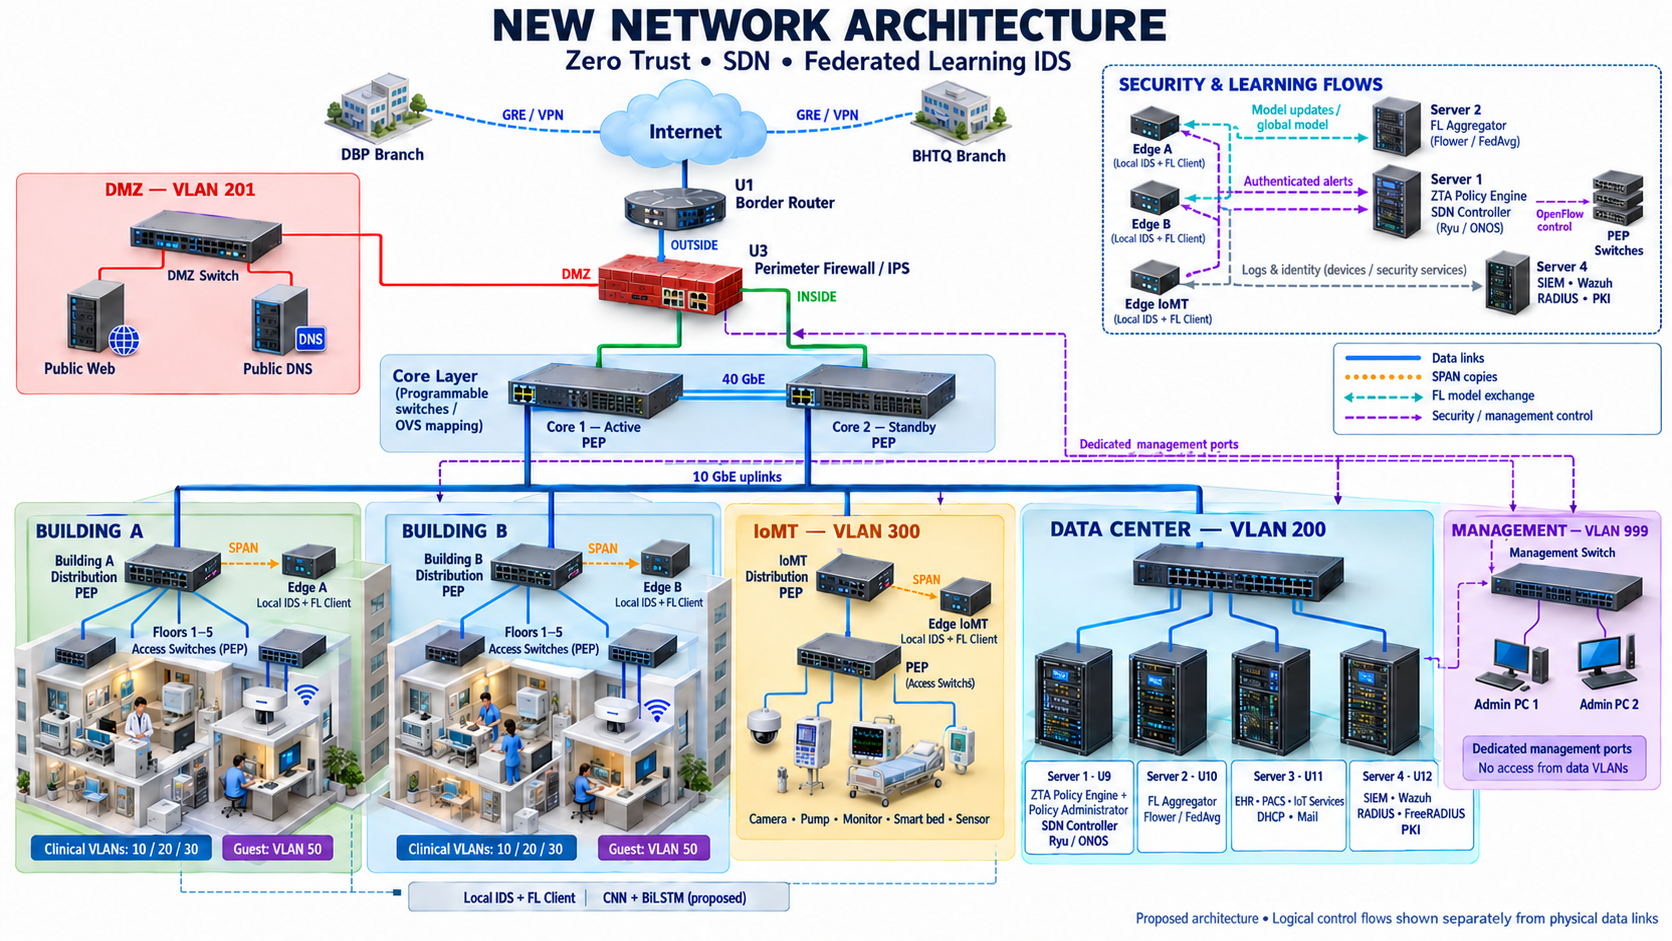
\includegraphics[width=0.96\textwidth]{graphics/architecture-overview.png}
  \caption{Overall FL-IDS + ZTA-SDN architecture for the segmented hospital network.}
  \label{fig:system_architecture}
\end{figure}

Within this graduation thesis, the system scope is structured into clear hardware/virtualization boundaries and departmental security zones, summarized in Table~\ref{tab:vlan_zones}.

\begin{table}[htbp]
  \centering
  \caption{Logical hospital network segmentation across zones and VRFs.}
  \label{tab:vlan_zones}
  \begin{tabular}{@{}l l l p{5.8cm}@{}}
    \toprule
    \textbf{Zone / VRF} & \textbf{VLAN IDs} & \textbf{Subnet Range} & \textbf{Primary Role and Security Policy} \\
    \midrule
    Clinical Zone & 10, 20, 30, 50, 60, 80 & \texttt{10.10.x.0/24} & Reception, Doctors, ICU, Wards, Pediatrics, Outpatient EMR clients; OOB access blocked via ingress ACLs. \\
    Paraclinical Zone & 110, 120, 130 & \texttt{10.20.x.0/24} & Laboratory, Diagnostic Imaging (PACS/DICOM), Pharmacy terminals; restricted server-only flows. \\
    Server Farm & 210, 220, 230, 240 & \texttt{10.30.x.0/24} & HIS/EMR app servers, PACS/LIS storage, Identity (AD/LDAP), SIEM/Monitoring. \\
    DMZ & 310, 320 & \texttt{172.16.x.0/24} & Patient Web Portal, OWASP CRS WAF, Reverse Proxy, DMZ IDS/FL edge sensor. \\
    SDN Control & 400 & \texttt{10.40.0.0/24} & OpenFlow control plane, PDP policy engine, FL aggregation server. \\
    OOB Management & 999 & \texttt{10.99.99.0/24} & Isolated device SSH management, NetBox/Ansible automation node, Tailscale bastion. \\
    \bottomrule
  \end{tabular}
\end{table}

\textbf{Scope Boundaries:}
\begin{itemize}[leftmargin=1.8em, itemsep=4pt]
  \item \textbf{Testbed Emulation:} The network core, distribution, access switches, edge firewall, and Linux service servers are emulated in GNS3 and VMware virtualized hosts using enterprise-representative images (Cisco IOSv/IOSvL2, ASAv, and Ubuntu Linux) with Infrastructure-as-Code pipelines stored in the project repository (\texttt{hospital-zta-sdn-fl}).
  \item \textbf{Detection and Mitigation Focus:} The FL-IDS evaluates both standard benchmark intrusion datasets and synthetic hospital-like attack traffic (e.g., port scanning, brute-force SSH, web exploitation, DICOM/clinical lateral movement). Compliance auditing is scoped to technical network/system controls rather than legal hospital accreditation.
\end{itemize}

\section{Contributions of the Thesis}
\label{sec:contributions}

The principal engineering and research contributions of this thesis are summarized as follows:

\begin{enumerate}[leftmargin=1.8em, itemsep=6pt]
  \item \textbf{Reproducible Zero-Touch Hospital Campus Infrastructure:} Designing a complete three-tier segmented hospital network backed by a single Source of Truth (NetBox), Terraform orchestration, and idempotent Ansible roles covering multi-VRF routing, two-layer OOB management protection, DNS/DHCP/Identity services, and OWASP CRS WAF deployment.
  \item \textbf{Integrated ZTA-SDN Enforcement and Out-of-Band Visibility:} Bridging enterprise Cisco SPAN traffic mirroring~\cite{ciscoSpan} and Suricata IDS/IPS~\cite{suricataIpsConcept} with an SDN Policy Decision Point that dynamically enforces quarantine and least-privilege rules at Policy Enforcement Points in alignment with NIST SP 800-207~\cite{rose2020zerotrust}.
  \item \textbf{Privacy-Preserving Multi-Zone FL-IDS Pipeline:} Implementing a federated intrusion detection workflow across logically isolated hospital domains (DMZ, Clinical, Paraclinical) using FedAvg~\cite{mcmahan2017communication} so collaborative detection improves without centralizing raw clinical network traffic~\cite{javeed2024federated,amiri2023sids}.
  \item \textbf{End-to-End Closed-Loop Validation Framework:} Delivering an automated, reproducible experimental testbed capable of quantifying classification accuracy, non-IID federated convergence, and real-time SDN quarantine latency under realistic attack scenarios.
\end{enumerate}

\section{Thesis Organization}
\label{sec:organization}

The remainder of this thesis is organized into five chapters:

\begin{itemize}[leftmargin=1.8em, itemsep=5pt]
  \item \textbf{Chapter~2 -- Theoretical Background and Infrastructure Design:} Reviews Zero Trust Architecture (NIST SP 800-207), SDN architecture, enterprise three-tier Campus design, IDS/IPS and WAF principles, Federated Learning foundations, and details our IaC-driven hospital network implementation.
  \item \textbf{Chapter~3 -- Federated Learning-Based Intrusion Detection System (FL-IDS):} Presents the deep learning model architecture, feature engineering over hospital and benchmark flow data, distributed FedAvg training pipeline, and edge inference design.
  \item \textbf{Chapter~4 -- Zero Trust Architecture and SDN Integration:} Details the coupling of Suricata/SPAN telemetry and FL-IDS alerts with the SDN PDP/PEP control loop, dynamic quarantine workflows, and policy enforcement rules.
  \item \textbf{Chapter~5 -- Experiments and Evaluation:} Describes the integrated testbed setup, attack simulation scenarios, FL-IDS classification benchmarks, SDN enforcement latency measurements, and comparative analysis.
  \item \textbf{Chapter~6 -- Conclusion and Future Work:} Summarizes key findings, discusses system limitations, and outlines future extensions for production healthcare deployments.
\end{itemize}
